% !TeX root = document.tex
%%%%%%%%%%%%%%%%%%%%%%%%%%%%%%%%%%%%%%%%%%%%%%%%%%%%%%%%%%%%%%%%%%%%%%%%%%%%%%%%%%%
%% This project aims to create the UFC template for presentation.                %%
%% author: Maurício Moreira Neto - Doctoral student in Computer Science (MDCC)   %%
%% contacts:                                                                     %%
%%    e-mail: maumneto@ufc.br                                                    %%
%%    linktree: https://linktr.ee/maumneto                                       %%
%%%%%%%%%%%%%%%%%%%%%%%%%%%%%%%%%%%%%%%%%%%%%%%%%%%%%%%%%%%%%%%%%%%%%%%%%%%%%%%%%%%

\documentclass{libs/ufc_format}
% Inserting the preamble file with the packages
%%%%%%%%%%%%%%%%%%%%%%%%%%%%%%%%%%%%%%%%%%%%%%%%%%%%%%%%%%%%%%%%%%%%%
%% This file contains the packages that can be used in the beamer. %%
%%%%%%%%%%%%%%%%%%%%%%%%%%%%%%%%%%%%%%%%%%%%%%%%%%%%%%%%%%%%%%%%%%%%%
% Package to fonts family
\usepackage[T1]{fontenc}
% Package to accentuation
\usepackage[utf8]{inputenc}
% Package to Portuguese language
\usepackage[brazil]{babel}
% Package to Figures
\usepackage{graphicx}
% Package to the colors
\usepackage{color}
% Package to the colors
\usepackage{xcolor}
% Packages to math symbols and expressions
\usepackage{amsfonts, amssymb, amsmath}
% Package to multiple lines and columns in table
\usepackage{multirow, array} 
% Package to create pseudo-code
% For more detail of this package: http://linorg.usp.br/CTAN/macros/latex/contrib/algorithm2e/doc/algorithm2e.pdf
\usepackage{algorithm2e}
% Package to insert code
\usepackage{listings} 
\usepackage{keyval}
% Package to justify text
\usepackage[document]{ragged2e}
% Package to manage the bibliography
\usepackage[backend=biber, style=numeric, sorting=none]{biblatex}
% Package to facilities quotations
\usepackage{csquotes}
% Package to use multicols
\usepackage{multicol}

\usepackage{booktabs}

\usepackage[flushleft]{threeparttable}

% Inserting the references file
\bibliography{references.bib}

% Title
\title[short title]{\huge\textbf{Título da Apresentação}}
% Subtitle
\subtitle{Subtítulo da Apresentação}
% Author of the presentation
\author{Otto Sousa}
% Institute's Name
\institute[UFC]{
    % email for contact
    \normalsize{\email{ottolopes20@gmail.com}}
    \newline
    % Department Name
    \department{Departamento de Engenharia de Teleinformática}
    \newline
    % university name
    \ufc
}
% date of the presentation
\date{\today}


%%%%%%%%%%%%%%%%%%%%%%%%%%%%%%%%%%%%%%%%%%%%%%%%%%%%%%%%%%%%%%%%%%%%%%%%%%%%%%%%%%
%% Start Document of the Presentation                                           %%               
%%%%%%%%%%%%%%%%%%%%%%%%%%%%%%%%%%%%%%%%%%%%%%%%%%%%%%%%%%%%%%%%%%%%%%%%%%%%%%%%%%
\begin{document}
% insert the code style
%%%%%%%%%%%%%%%%%%%%%%%%%%%%%%%%%%%%%%%%%%%%%%%%%%%%%%%%%%%%%%%%%%%%%%%%%%%%%%%%%%%
%% This file contains the style of the codes show in slides.                     %%
%% The package used is listings, but it possible to used others.                 %%
%%%%%%%%%%%%%%%%%%%%%%%%%%%%%%%%%%%%%%%%%%%%%%%%%%%%%%%%%%%%%%%%%%%%%%%%%%%%%%%%%%%

% color used in the code style
\definecolor{codegreen}{rgb}{0,0.6,0}
\definecolor{codegray}{rgb}{0.5,0.5,0.5}
\definecolor{codepurple}{rgb}{0.58,0,0.82}
\definecolor{codebackground}{rgb}{0.95,0.95,0.92}

% style of the code!
\lstdefinestyle{codestyle}{
    backgroundcolor=\color{codebackground},   
    commentstyle=\color{codegreen},
    keywordstyle=\color{magenta},
    numberstyle=\tiny\color{codegray},
    stringstyle=\color{codepurple},
    basicstyle=\ttfamily\footnotesize,
    frame=single,
    breakatwhitespace=false,         
    breaklines=true,                 
    captionpos=b,                    
    keepspaces=true,                 
    numbers=left,                    
    numbersep=5pt,                  
    showspaces=false,                
    showstringspaces=false,
    showtabs=false,                  
    tabsize=2,
    title=\lstname 
}

\lstset{style=codestyle}


%% ---------------------------------------------------------------------------
% First frame (with tile, subtitle, ...)
\begin{frame}{}
    \maketitle
\end{frame}

%% ---------------------------------------------------------------------------
% Second frame
\begin{frame}{Sumário}
    \begin{multicols}{2}
        \tableofcontents
    \end{multicols}
\end{frame}

%% ---------------------------------------------------------------------------
% This presentation is separated by sections and subsections
\section{Seção I}
\begin{frame}{Explicações}
    % itemize
    Este é um template que pode ser utilizado para:
    \begin{itemize}
        \item Apresentação de Trabalhos Acadêmicos
        \item Apresentação de Disciplinas
        \item Apresentações de Teses e Dissertações
    \end{itemize}

    \vspace{0.4cm} % vertical space
    
    % enumeration
    Para utilizar este template corretamente é importante que:
    \begin{enumerate}
        \item Tenha conhecimento mínimo sobre LaTeX
        \item Ler os comentários no template (explicações)
        \item Ler o README.md (documentação)
    \end{enumerate}

    \vspace{0.2cm}

    \example{Este é um texto de exemplo!} \emph{Texto de Ênfase!}
\end{frame}

%% ---------------------------------------------------------------------------
\subsection{Subseção I}
\begin{frame}{Criando Blocos}
    % Blocks styles
    \begin{block}{Bloco Padrão}
        Texto do corpo do bloco.
    \end{block}

    \begin{alertblock}{Bloco de Alerta}
        Texto do corpo do bloco.
    \end{alertblock}

    \begin{exampleblock}{Bloco de Exemplo}
        Texto do corpo do bloco.
    \end{exampleblock}   
\end{frame}

%% ---------------------------------------------------------------------------
\subsection{Subseção II}
\begin{frame}{Criando Caixas}
    \successbox{testando o success box}

    \pause

    \alertbox{testando o alert box}

    \pause

    \simplebox{testando o simple box}
\end{frame}

%% ---------------------------------------------------------------------------
\subsection{Subseção III}
\begin{frame}{Criando Algoritmos (Pseudocódigo)}
    \begin{algorithm}[H]
        \SetAlgoLined
        \LinesNumbered
        \SetKwInOut{Input}{input}
        \SetKwInOut{Output}{output}
        \Input{x: float, y: float}
        \Output{r: float}
        \While{True}{
          r = x + y\;
          \eIf{r >= 30}{
           ``O valor de $r$ é maior ou iqual a 10.''\;
           break\;
           }{
           ``O valor de $r$ = '', r\;
          }
         } 
         \caption{Algorithm Example}
    \end{algorithm}
\end{frame}

%% ---------------------------------------------------------------------------

\begin{frame}{Inserindo Algoritmos}
    \lstset{language=Python}
    \lstinputlisting[language=Python]{code/main.py}
\end{frame}

%% ---------------------------------------------------------------------------
\begin{frame}{Inserindo Algoritmos}
    \lstinputlisting[language=C]{code/source.c}
\end{frame}

%% ---------------------------------------------------------------------------
\begin{frame}{Inserindo Algoritmos}
    \lstinputlisting[language=Java]{code/helloworld.java}
\end{frame}

%% ---------------------------------------------------------------------------
\begin{frame}{Inserindo Algoritmos}
    \lstinputlisting[language=HTML]{code/index.html}
\end{frame}

%% ---------------------------------------------------------------------------
% This frame show an example to insert multicolumns


\section{Multicolunas}
\begin{frame}{Seção II - Multicolunas}
    \begin{columns}{}
        \begin{column}{0.5\textwidth}
            \justify
            É possível colocar mais de uma coluna utilizando os comandos de $\backslash$begin\{column\}\{\} e $\backslash$end\{column\}
        \end{column}
        \begin{column}{0.5\textwidth}
            \justify
            Porém, o espaçamento deve ser proporcional entre as colunas para que estas colunas não entrem em coflito. O espaçamento é dado pelo segundo argumento do $\backslash$begin.
        \end{column}
    \end{columns}    
\end{frame}

%% ---------------------------------------------------------------------------
% This frame show an example to insert figures



\section{Introdução}
\begin{frame}{Introdução}
    % itemize
    
    Um dispositivo \textit{datalogger} é um sistema embarcado que realiza que realiza e armazena leituras do ambiente em que está presente por meio de sensores.

    % Demonstrar o processo de desenvolvimento do hardware de um sistema embarcado usando como exemplo a concepção e desenvolvimento de um dispositivo \textit{datalogger}
    
    % Este é um template que pode ser utilizado para:
    % \begin{itemize}
    %     \item Apresentação de Trabalhos Acadêmicos
    %     \item Apresentação de Disciplinas
    %     \item Apresentações de Teses e Dissertações
    % \end{itemize}

    % % \vspace{0.4cm} % vertical space
    
    % % enumeration
    % Para utilizar este template corretamente é importante que:
    % \begin{enumerate}
    %     \item Tenha conhecimento mínimo sobre LaTeX
    %     \item Ler os comentários no template (explicações)
    %     \item Ler o README.md (documentação)
    % \end{enumerate}

    % \vspace{0.2cm}

    % \example{Este é um texto de exemplo!} \emph{Texto de Ênfase!}
\end{frame}

\begin{frame}{Introdução}
    Métodos de recuperação dos dados coletados: 
    
    \begin{itemize}
        \item Manual - Um operador deve ir ao local de instalação. Preço unitário acessível;  
        \item Automatizada - Envio de informações via interface sem fio. Eleva o preço unitário do \textit{datalogger}.
    \end{itemize}

\end{frame}






\begin{frame}{Objetivo geral}
    % itemize
    Desenvolver os esquemáticos eletrônicos e leiaute da placa de circuito impresso de um \textit{datalogger} de baixo custo, com interfaces Wi-Fi e \textit{Bluetooth}, que possa realizar medições de temperatura, umidade e luminosidade. 
    
    % \begin{itemize}
    %     \item Recuperação manual de dados;
    %     \item Recuperação automatizada de dados;
    % \end{itemize}
    
    
    
    % Demonstrar o processo de desenvolvimento do hardware de um sistema embarcado usando como exemplo a concepção e desenvolvimento de um dispositivo \textit{datalogger}
    
    % Este é um template que pode ser utilizado para:
    % \begin{itemize}
    %     \item Apresentação de Trabalhos Acadêmicos
    %     \item Apresentação de Disciplinas
    %     \item Apresentações de Teses e Dissertações
    % \end{itemize}

    % % \vspace{0.4cm} % vertical space
    
    % % enumeration
    % Para utilizar este template corretamente é importante que:
    % \begin{enumerate}
    %     \item Tenha conhecimento mínimo sobre LaTeX
    %     \item Ler os comentários no template (explicações)
    %     \item Ler o README.md (documentação)
    % \end{enumerate}

    % \vspace{0.2cm}

    % \example{Este é um texto de exemplo!} \emph{Texto de Ênfase!}
\end{frame}



\begin{frame}{Objetivos específicos}

Os objetivos específicos desse trabalho são:
    
\begin{itemize}
    \item Análise de soluções existentes;
    \item Levantamento de escopo e especificações;
    \item Criação de arquitetura;
    \item Seleção de componentes e criação de esquemáticos eletrônicos;
    \item Desenvolvimento de PCI;
    \item Mensuração dos custos;
    \item Definição da autonomia típica;
    \item Comparativo de mercado.
\end{itemize}
    
    
\end{frame}

% \section{Fundamentação Teórica}

% \begin{frame}
    
%     \centering
%     \color{blue_theme}\huge{{Fundamentação}}

% \end{frame}


\begin{frame}{Sistemas Embarcados}
    \begin{block}{Definição}
        
        São sistemas computacionais que são parte integrante de 
        um produto ou ferramenta e são limitados em tamanho, consumo, 
        poder de processamento e custo. 

        
    \end{block}

    % \vfill{}

    \vspace{30pt}

    Produtos que possuem um sistema embarcado são:

    \begin{itemize}
        % \item Controles remotos;
        \item Brinquedos;
        \item Eletrodomésticos;
        \item Automóveis;
    \end{itemize}


\end{frame}

%% ---------------------------------------------------------------------------

% \begin{frame}{Sistemas Embarcados}

% \end{frame}

\begin{frame}{Sistemas Embarcados}

    Estrutura básica:
    \begin{itemize}
        \item Unidade de fornecimento de energia elétrica;
        \item Interfaces de entrada e saída para interação;
        \item Memórias de dados e de programa;
        \item Interfaces de comunicação;
        \item \textbf{Unidade de processamento};
        
    \end{itemize}
\end{frame}



\begin{frame}{Tecnologias de processadores}

    \begin{block}{Definição}
        Maneira como a unidade de processamento é 
        organizada para executar instruções.
    \end{block}


    \begin{itemize}
        \item Processadores de Uso Geral
        \item Processadores Especializados
        \begin{itemize}
            \item Microcontroladores;
            \item DSPs.
        \end{itemize}
        \item Processadores Dedicados
        \begin{itemize}
            \item ASICs
            \item FPGAs
        \end{itemize}
        \item System-On-A-Chip
    \end{itemize}



\end{frame}

% \begin{frame}{Processadores de uso geral}

%     \begin{itemize}
%         \item Dispositivos programáveis;
%         \item Possuem grande número de instruções;
%         \item Pode executar múltiplos processos simultaneamente;
%         \item Menor tempo de desenvolvimento;
%         \item Maior custo unitário.
        
%     \end{itemize}

% \end{frame}

% \begin{frame}{Processadores especializados}

%     \begin{itemize}
%         \item Número de instruções reduzidos;
%         \item Menor custo e poder de processamento;
%         \item Menor custo unitário; 
%         \item Maior tempo de desenvolvimento;
%         \item Podem ser programados;
%     \end{itemize}

    
% \end{frame}


% \begin{frame}{Processadores especializados}

%     \begin{itemize}
%         \item Microcontroladores
            
%             \begin{itemize}
%                 \item CPU, RAM, I/O, UART, I²C e SPI em um mesmo chip;
%                 \item Otimizado para aplicações de controle;
%                 \item Não lida com grande volume de dados ou cálculos complexos;
%             \end{itemize}
            
%         \item \textit{Digital Signal Processors}
            
%             \begin{itemize}
%                 \item Semelhante a microcontroladores;
%                 \item Realiza operações de adição e multiplicação mais eficientemente;
%                 \item Processa grande volume de dados;
%                 \item Otimizado para processamento de sinais;
%             \end{itemize}
            
%     \end{itemize}

    
% \end{frame}




% \begin{frame}{Processadores dedicados}

% \begin{itemize}
%     \item Não programáveis;
%     \item Implementa instruções para uma aplicação em específica;
%     \item Maior custo de desenvolvimento;
% \end{itemize}

% \end{frame}


% \begin{frame}{Processadores dedicados}

%     \begin{itemize}
%         \item Application Specific Integrated Circuit (ASIC)
%         \begin{itemize}
%             \item Circuito integrado de aplicação específica;
%             \item Possui a lógica necessária para execução de tarefas;
%             \item Não permite reconfiguração da lógica implementada;
%         \end{itemize}
        
%         \item Field Programmable Gate Array
        
%             \begin{itemize}
%                 \item Semelhante ao ASIC;
%                 \item Matriz de blocos lógicos reconfiguráveis;
%                 \item Conexões programáveis interligam os blocos da matriz;
%                 \item Permite a reconfiguração da lógica implementada;
%             \end{itemize}
%     \end{itemize}

% \end{frame}


% \begin{frame}{System-On-A-Chip}
%     \begin{itemize}

%     \item Circuito integrado formado por diversos módulos que compõem um sistema computacional;
    
%     \item Visa reduzir o número de CIs utilizados em um sistema embarcado;
    
%     \item Implementa módulos além de CPU, RAM e I/Os;
    
%         \begin{itemize}
%             \item Módulos de comunicação sem fio; 
%             \item Módulos de processamento de sinais.
%         \end{itemize}
    
%     \end{itemize}
% \end{frame}



\begin{frame}{Desafios de Projeto}

    \begin{itemize}
    
        \item Realizar uso eficiente dos recursos computacionais disponíveis;
        
        
        \item Um sistema embarcado deve atingir a dependabilidade;
        
        \begin{itemize}
            \item Segurança da informação;
            \item Confidencialidade;
            \item Operação segura;
            \item Confiabilidade;
            \item Reparabilidade;
        \end{itemize}
        
        
        
        
    \end{itemize}
    
    
    
    

    
\end{frame}





% \subsection{Subseção I}
% \begin{frame}{Criando Blocos}
%     % Blocks styles
%     \begin{block}{Bloco Padrão}
%         Texto do corpo do bloco.
%     \end{block}

%     \begin{alertblock}{Bloco de Alerta}
%         Texto do corpo do bloco.
%     \end{alertblock}

%     \begin{exampleblock}{Bloco de Exemplo}
%         Texto do corpo do bloco.
%     \end{exampleblock}   
% \end{frame}

\section{Metodologia}


\begin{frame}
    
    \centering
    \color{blue_theme}\huge{{Metodologia}}

\end{frame}




\begin{frame}{Soluções existentes}


    
        \begin{itemize}
            \item Busca de dispositivos com as seguintes propriedades:
                \begin{itemize}
                    \item Leitura de umidade e temperatura;
                    \item Comunicação sem fio;
                    \item Opção de alimentação por bateria;
                \end{itemize}
            
            \item Análise de custo e propriedades de soluções existentes.
        \end{itemize}
    
    
	
    \end{frame}
    
    
    \begin{frame}
    
            \begin{table}[!h]\label{tab:dataloggers_novos}
        	
        	\captionsetup{width=8cm}%Deixe da mesma largura que a tabela
        	\caption{\textit{Dataloggers: Preços e Mercados}}%
        % 	\begin{threeparttable}
        	\resizebox{\textwidth}{!}{
        	
        		\begin{tabular}{cccccc}
        			\toprule
                    % \hline
        			Modelo & Fabricante & Preço (R\$) & Mercado & Nível de Proteção & Interface sem Fio \\
        			\midrule \midrule
                    RCW-360        & Elitech            &  1.499,00 & Nacional    & IP64/IP65 & WiFi \\
                    EL-WiFi-TH     & Lascar Electronics &  1.305,14 & Estrangeiro & IP55  & WiFi    \\
                    TandD RTR-507B & TandD              &  2.242,57 & Estrangeiro & IP64  & Interface Própria    \\
                    160 TH         & testo              &  2.842,00 & Nacional    & IP20 & WiFi
                    \\ 
        		    \bottomrule
        		\end{tabular}%
        	
        	}
        	
        % 	\begin{tablenotes}
        	
        
        %     {%
        % 	\tiny{o autor.}%
        	    \tiny{tiny: o autor}\\
        	
        %     }
        % 	\end{tablenotes}
            % \end{threeparttable}
            \end{table}
    
            \begin{table}[!h]\label{tab:dataloggers_novos_propriedades}
        	
        	\captionsetup{width=7cm}%Deixe da mesma largura que a tabela
        	\caption{\textit{Dataloggers: Propriedades}}%
        	\resizebox{\linewidth}{!}{
        % 	\IBGEtab{}{%
        		\begin{tabular}{ccccccc}
        			\toprule
        			Modelo & Dimensões & Autonomia & Faixa de Leitura (ºC) & Precisão (ºC) & Umidade Relativa (\%) & Precisão(\%)\\
        			\midrule \midrule
                   RCW-360        & Não informado   & 3 meses       & -35 a 80 & 0,5 & 0 a 99 & 5    \\
                   EL-WiFi-TH     & 82 x 70 x 23 mm & 6 meses       & -20 a 60 & 0,3 & 0 a 100 & 2    \\
                   TandD RTR-507B & 62 x 47 x 19 mm & 10 meses      & -25 a 70 & 0,3 & 0 a 99  & 2,50 \\
                   160 TH         & 76 x 64 x 22 mm & Não informado & -30 a 50 & 0,1 & 0 a 100 & 2   
                    \\
        	    \bottomrule
        		\end{tabular}%
        	}
                \tiny{tiny: o autor}\\
            \end{table}
\end{frame}

\begin{frame}{Escopo de Projeto}

    \begin{block}{Escopo de projeto}
        Desenvolvimento um \textit{datalogger} de baixo custo que seja capaz de ler temperatura, umidade relativa e luminosidade de um ambiente em que ele estiver instalado. Deve ser possível que essas leituras sejam realizadas periodicamente de forma que o intervalo mínimo entre cada possa estar na casa dos segundos e devem ser armazenadas em uma mídia de armazenamento de massa removível para facilitar o resgate dessas informações posteriormente.
    \end{block}
    
\end{frame}





\begin{frame}{Especificações técnicas}

    \begin{enumerate}
        \item Possuir a capacidade de ler a temperatura do ambiente;
        \item Possuir a capacidade de ler a umidade relativa do ambiente;
        \item Possuir a capacidade de ler o nível de luminosidade do ambiente;
        \item Possuir alternativa de alimentação direta ou via bateria;
        \item Leitura de sensores via interfaces I²C, SPI e/ou UART;
        % \item Formatação dos dados lidos dos sensores para auxiliar no envio e/ou coleta;
        \item Persistir os dados em um cartão SD para facilitar a recuperação manual dos dados coletados;
        \item Persistência dos dados coletados por no mínimo 45 dias;
        % \item Interface de comunicação via rádio LoRa;
        % \item Envio periódico dos dados guardados via LoRaWan;
        \item Possuir interface de interação com o usuário;
        % \item Permitir a configuração da taxa de amostragem das variáveis lidas;
        \item Permitir o envio de dados coletados via interface de comunicação sem fio;
    \end{enumerate}
    
\end{frame}


\begin{frame}{Arquitetura de Hardware}
    
     \begin{itemize}
     \item Unidade de processamento;
     \item Sensor de luminosidade;
     \item Sensor de temperatura; 
     \item Sensor de umidade;
     \item Unidade de alimentação;
     \item Unidade de interface de usuário;
    %  \item Unidade de interface de comunicação USB;
     \item Unidade de leitura e escrita de dados em cartão SD;
     
    
      \end{itemize}
 \end{frame}
      
\begin{frame}{Arquitetura de Hardware}

    \begin{figure}
        \centering
        \caption{Diagrama de blocos.}
        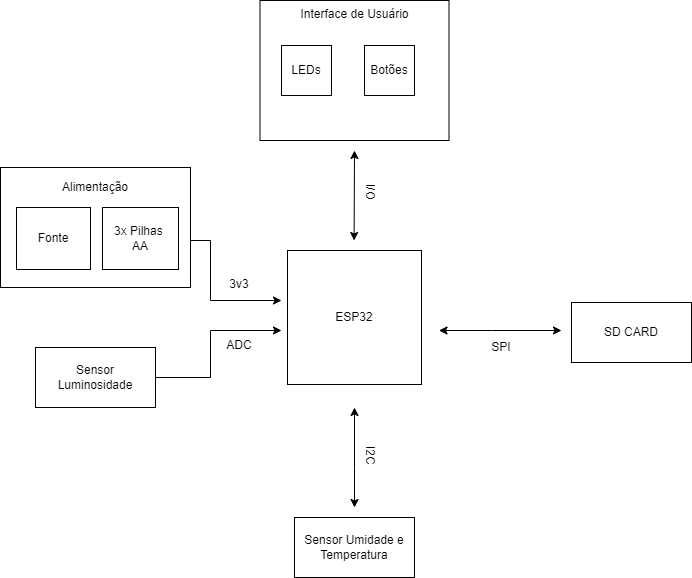
\includegraphics[scale=0.3]{figuras/cap3/datalogger_tcc.png}
        \source{Elaborado pelo autor (2022)}
        \label{fig:block_diagram}
    \end{figure}
    
\end{frame}


\begin{frame}{Seleção de Componentes}

    \begin{block}{Critérios}
        Foram definidos alguns critérios para se escolher um componente:
        
        \begin{enumerate}
            
            \item Tempo de suporte de ciclo de vida maior 10 anos p/ componentes ativos;
            \item Selecionar componentes passivos com propriedades que facilitem sua substituição;
            \item Possuir mais de uma solução para cada componente passivo;
            
        \end{enumerate}
    
        
    \end{block}

\end{frame}

\begin{frame}{Microcontrolador}

\only<1>{

    \framesubtitle{Definição}

    \begin{columns}
            
        \column{0.4\textwidth}
        \justify 
        \begin{itemize}
            \item ESP32-S3-WROOM-1-N8
            \begin{itemize}
                \item Baixo custo unitário;
                \item 8MB de \textit{Flash} e 36 GPIOs;
                \item Wi-Fi 2.4GHz e BLE Radio;
                \item ADC 10-bits;
                \item 12 anos de suporte de ciclo de vida.
                % \item 
            \end{itemize}
        \end{itemize}
        
        \column{0.6\textwidth}
        \justify
        \begin{figure}
            % \centering
            \caption{Diagrama de blocos do módulo}
            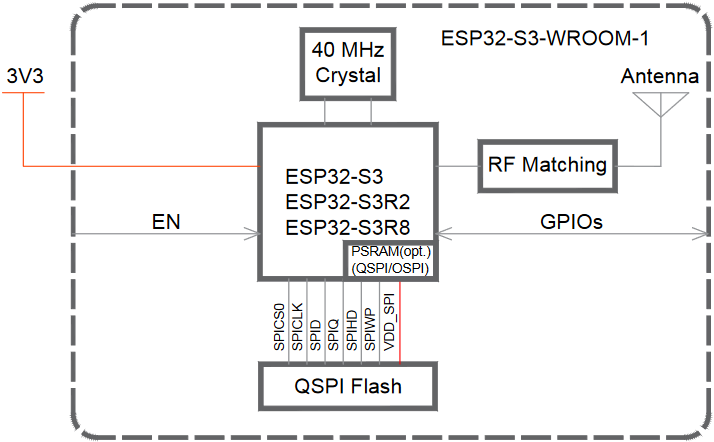
\includegraphics[scale=0.35]{figuras/cap3/modulo_block_diagram.png}
            \source{Espressif Systems}
            \label{fig:soc_esp32}
        \end{figure}
    \end{columns}
}



\only<2>{
\framesubtitle{Esquemático}

    \begin{figure}
        \centering
        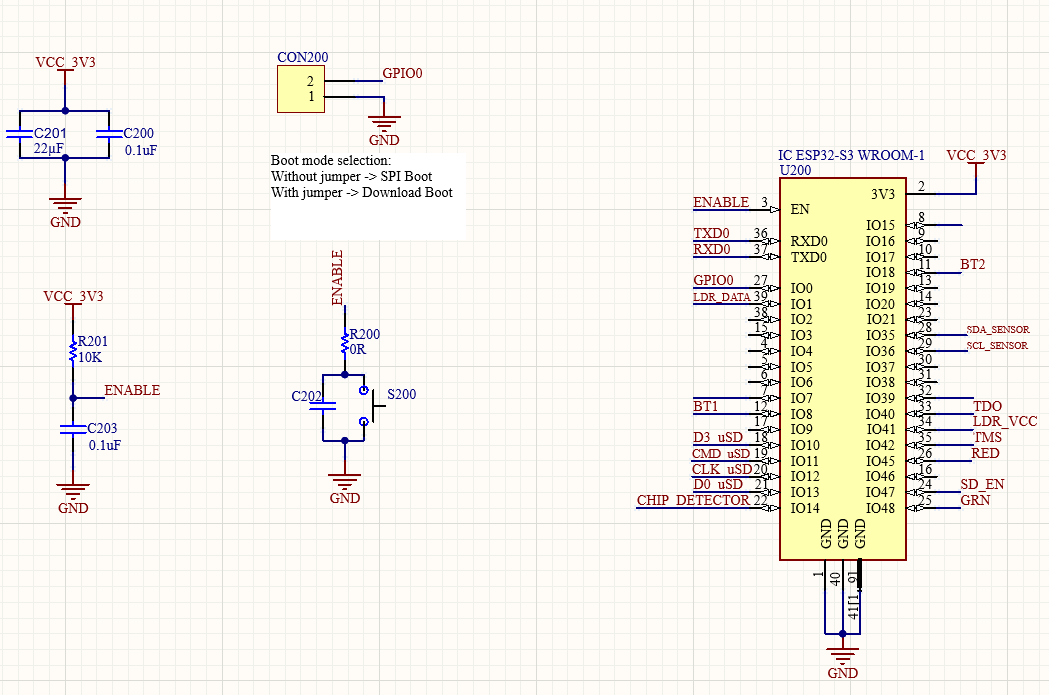
\includegraphics[width=0.85\textwidth]{figuras/cap3/esquematicos/controller.png}
        \source{Elaborado pelo autor}   
    \end{figure}
}





\end{frame}

\begin{frame}{Sensores}

    \only<1>{
        \framesubtitle{HDC1080}
        \begin{columns}
                \column{0.45\textwidth}
                \centering
                \begin{itemize}
                    \item TI HDC1080
                    \begin{itemize}
                        \item $\pm$2\% de precisão de umidade relativa;
                        \item $\pm$0.2 °C precisão de temperatura;
                        \item 1.3 $\mu$A p/ leitura e 100 nA hibernação;
                        % \item Interface I²C
                    \end{itemize}
                \end{itemize}
                
                \column{0.55\textwidth}
                \centering

                \begin{figure}
                    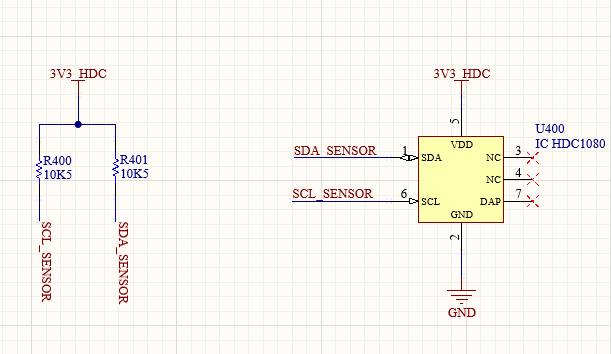
\includegraphics[width=\textwidth]{figuras/cap3/esquematicos/temp_sensor.png}
                \end{figure}
                
                
        \end{columns}

    }




    \only<2>{

        \framesubtitle{LDR}
        \begin{columns}
            \column{0.5\textwidth}

            \begin{itemize}
                \item \textit{Light Dependant Resistor} (LDR)
                \begin{itemize}
                    \item Baixo custo;
                    \item 10 a 10.000 lux;
                    \item Necessita de ADC;
                \end{itemize}
            \end{itemize}
            
            \column{0.5\textwidth}
                       
                \begin{figure}
                    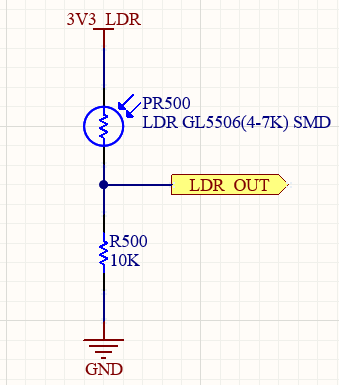
\includegraphics[width=0.7\textwidth]{figuras/cap3/esquematicos/light_sensor.png}
                \end{figure}
            
            
            
            
        \end{columns}

    }

    
\end{frame}

\begin{frame}{Interface de usuário e suporte MicroSD}


    \only<1>{
        \begin{columns}
            \column{0.45\textwidth}
                \vspace{-40pt}
                \centering
                \begin{itemize}
                    \item \textit{LEDs} e botões táteis
                    \begin{itemize}
                        \item LEDs genéricos vermelho e verde;
                        \item Dois botões táteis;
                    \end{itemize}
                
                    \vspace{50pt}
                
                    \item Suporte microSD
                
                \end{itemize}
                



                % \begin{itemize}

                
                % % \begin{itemize}
                % %     \item
                % % \end{itemize}
                % \end{itemize}


                \column{0.55\textwidth}
                \centering

                


                \begin{figure}
                    \centering
                    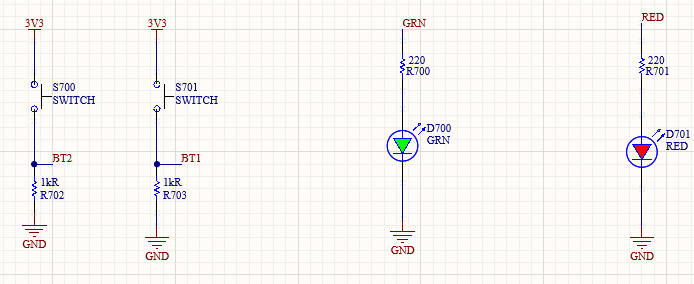
\includegraphics[width=\textwidth]{figuras/cap3/esquematicos/user_interface.png}
                    % \source{Elaborado pelo autor.}
                \end{figure}


                \begin{figure}
                    \centering
                    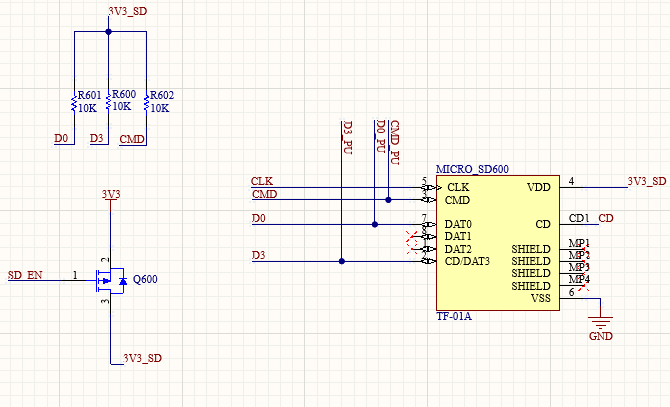
\includegraphics[width=\textwidth]{figuras/cap3/esquematicos/sdcard.png}
                    \vspace{-15pt}
                    \source{Elaborado pelo autor.}
                \end{figure}
        
        \end{columns}
    }

% \only<2>{

%     \framesubtitle{Esquemático}
%     \begin{columns}
%         \column{0.5\textwidth}
 
        
%         \column{0.5\textwidth}
                   

        
        
        
        
%     \end{columns}

% }


\end{frame}

\begin{frame}{Fonte de alimentação}

    \only<1>{
        \begin{block}{Requisitos}
            \begin{enumerate}
                \item Fornecer 3,3 V;
                \item Suportar alimentação por 4 pilhas;
                \item ``Chaveamento'' entre pilhas e alimentação direta;
            \end{enumerate}
        \end{block}
    }

% \framebreak
    \only<2>{

        % \begin{columns}
        %     \column{0.35\textwidth}
                % \vspace{3pt}
                \begin{itemize}
                    \item Circuito ``chaveador'' pilha-alimentação direta:
                    \begin{itemize}
                        \item MOSFET Canal P;
                        \item Resistor 10k$\Omega$;
                        \item Diodo \textit{schottky};
                    \end{itemize}
                    \item \textit{Schottky} ON NSR0320MW2T1
                    \begin{itemize}
                        \item Tensão direta típica: 0,3 V;
                    \end{itemize}
                    
                \end{itemize}
            % \column{0.65\textwidth}
                \vspace{-7pt}
                \begin{figure}
                    \centering
                    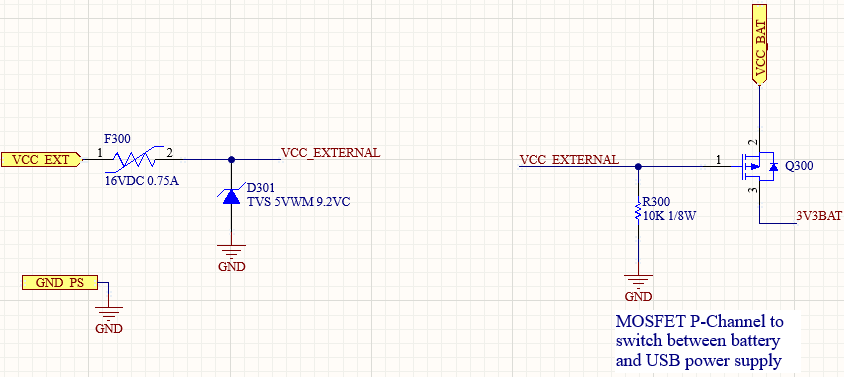
\includegraphics[width=0.8\textwidth]{figuras/cap3/esquematicos/power_1.png}
                    % \source{Elaborado pelo autor.}
                \end{figure}




        % \end{columns}

    }


% \framebreak
    
        \only<3>{        
            \begin{block}{Regulação de tensão}

            Quatro pilhas do tipo AA fornecem até 6V de tensão. É preciso reduzi-lá para 3,3 V, nível de tensão operacional dos demais componentes.

            \end{block}

            \begin{columns}
                    
                    \column{0.5\linewidth}
                    \centering
                    \begin{itemize}
                        \item Regulador Linear
                        \begin{itemize}
                            \item Baixo custo;
                            % \item Menor uso de componentes;
                            \item Baixa complexidade;
                            \item Baixa eficiência;
                            \item \textit{Step-down};
                        \end{itemize}
                    \end{itemize}
                    
                    \column{0.5\linewidth}
                    
                    \begin{itemize}
                        \item Regulador Chaveado
                        \begin{itemize}
                            \item Maior custo;
                            % \item Maior uso de componentes;
                            \item Alta complexidade;
                            \item Alta eficiência;
                            \item \textit{Step-up} ou \textit{Step-down};
                        \end{itemize}
                    \end{itemize}
                    
            \end{columns}

        }    


% \framebreak
        \only<4>{
            \begin{block}{Regulador linear \textit{low-dropout}}

            Reguladores lineares que podem regular a tensão de saída mesmo quando a tensão entrada se aproximar muito da tensão de saída.

            \end{block}

            \begin{columns}
                \column{0.45\textwidth}
                    \begin{itemize}
                        \item Diodes AP2114HA-3.3TRG1
                        \begin{itemize}
                            \item Suporta até 6,5 V de entrada;
                            \item 3,3 V fixo como saída;
                            \item Queda típica de 0,1 V;
                        \end{itemize}
                    \end{itemize}
                \column{0.55\textwidth}
                    
                    \begin{figure}
                        \centering
                        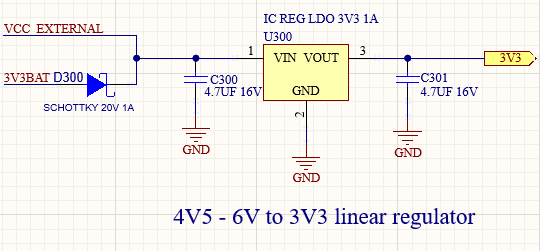
\includegraphics[width=\textwidth]{figuras/cap3/esquematicos/power_2.png}
                        \source{Elaborado pelo autor.}
                    \end{figure}   



                
            \end{columns}
            % \framebreak
        }    
\end{frame}



\begin{frame}{Design PCI}

    \only<1>{
    \begin{block}{Especificações}
    
    \begin{itemize}
        \item Dimensões aproximadas de 50x50 mm;
        \item Placa de duas camada;
    \end{itemize}
    \end{block}
    }
      
    
    % \framesubtitle{\textit{Stackup} PCI}
    \centering
    \only<2>{

    \begin{block}{\textit{Stackup PCI}}
        
        Define características e parâmetros do cobre e dielétrico de uma PCI.
    
    \end{block}
    \begin{figure}
        \centering
        
        
        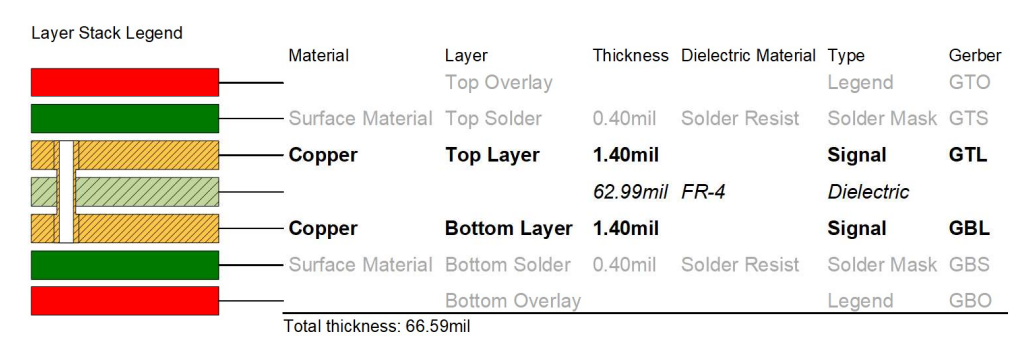
\includegraphics[width=0.7\linewidth]{figuras/cap3/pcb/pcb_stackup.png}
       
        % \includegraphics{}
        % \caption{}
        \scriptsize{Impedância típica: 50$\Omega$}
        % \caption{Particionamento Recomendado}
        \source{Elaborado pelo autor.}
        
        \label{fig:stackup_pci}
    \end{figure}
    
    }
    % \item Impedância típica - 50$\Omega$
    
    \only<3>{
    
    \framesubtitle{{Particionamento Funcional}}
    
    \begin{columns}
        \column{0.45\linewidth}
        \raggedleft
        \begin{itemize}
            \item Posição de componentes;
            \item Auxílio de roteamento;
            \item Redução EMI;
        \end{itemize}
        
        
        \column{0.55\linewidth}
        \raggedright
        \begin{figure}
            \centering
            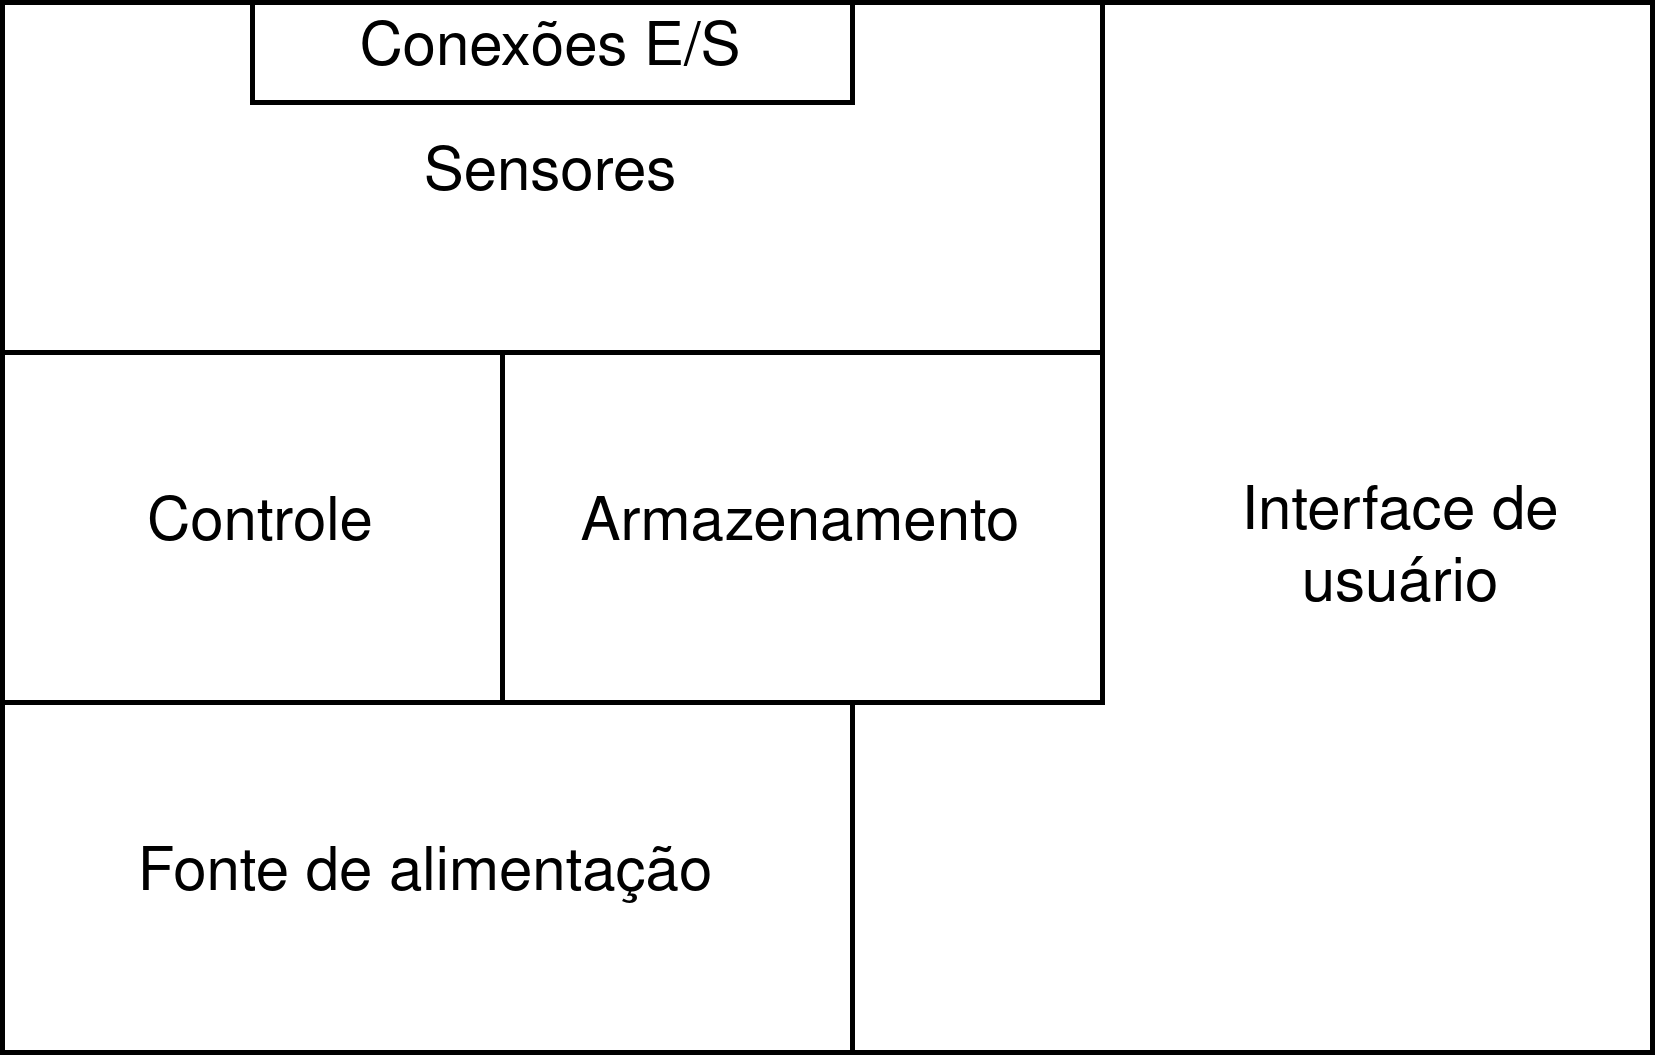
\includegraphics[width=\linewidth]{figuras/cap3/particionamento.drawio.PNG}
            % \caption{Caption}
            \source{Elaborado pelo autor.}
            \label{fig:my_label}
        \end{figure}
    
    \end{columns}

    }

    \only<4>{
    
    \framesubtitle{{Posicionamento}}
    
    \begin{figure}
        \centering
        \caption{\textit{PCB Placement}}
        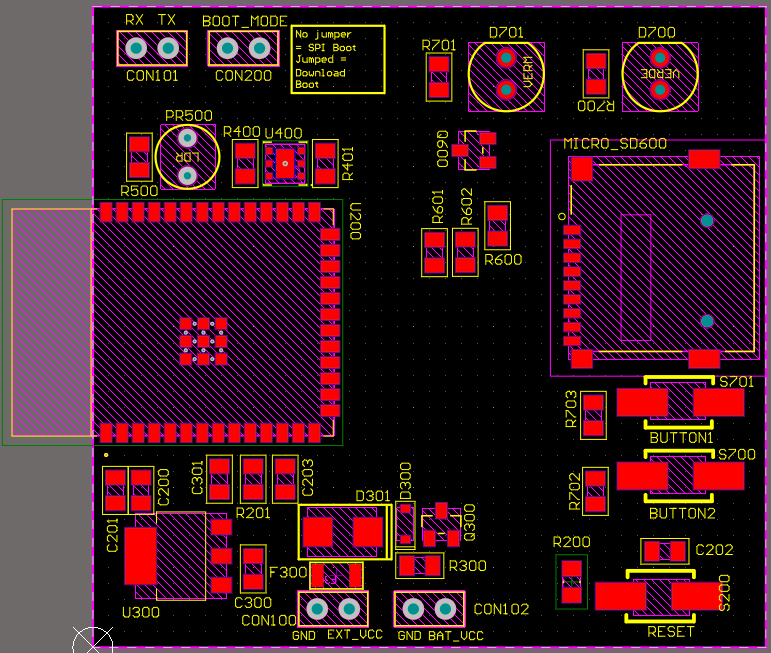
\includegraphics[width=0.6\linewidth]{figuras/cap3/pcb/pcb_no_route.png}
        \source{Elaborado pelo autor}
        \label{fig:pcb_placement}
    \end{figure}
    }

    \only<5>{

    \framesubtitle{{Roteamento}}

    \begin{columns}
        
        \column{0.4\linewidth}
        \centering
        \begin{itemize}
            \item Somente sinais inicialmente;
            \item Largura 10 mil;
        \end{itemize}
        
        \column{0.6\linewidth}
        \begin{figure}
            \centering
            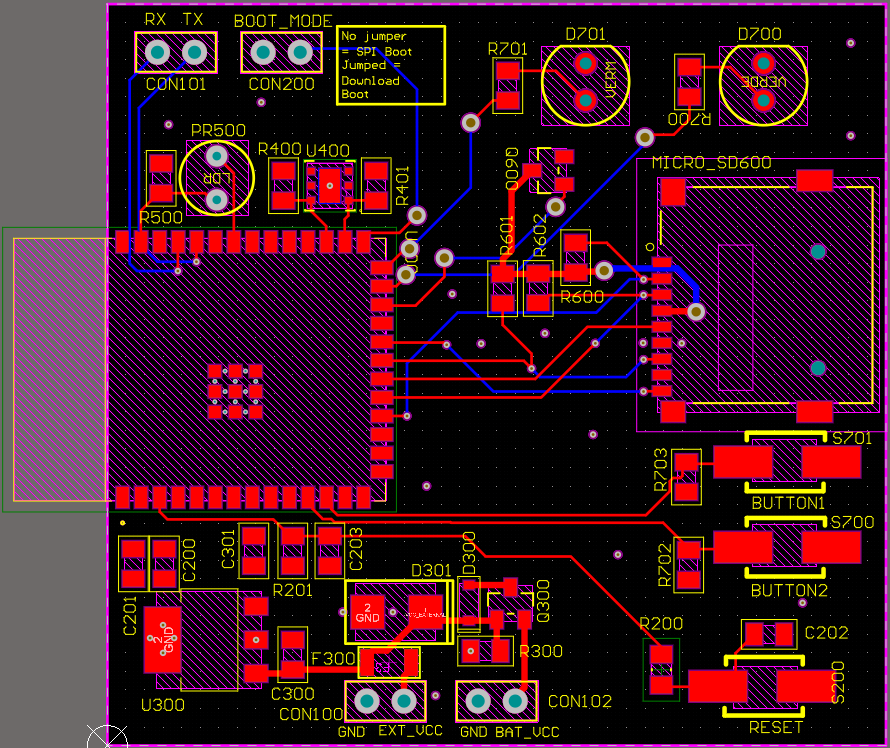
\includegraphics[width=\linewidth]{figuras/cap3/pcb/pcb_signlas_route.png}
            \source{Elaborado pelo autor}
        \end{figure}


    \end{columns}
    }

    \only<6>{

    \framesubtitle{{Roteamento}}

    \begin{columns}
        
        \column{0.4\linewidth}
        \centering
        \begin{itemize}
            \item Evita ciclos;
            \item Largura 20 mil;
        \end{itemize}
        
        \column{0.6\linewidth}
        \begin{figure}
            \centering
            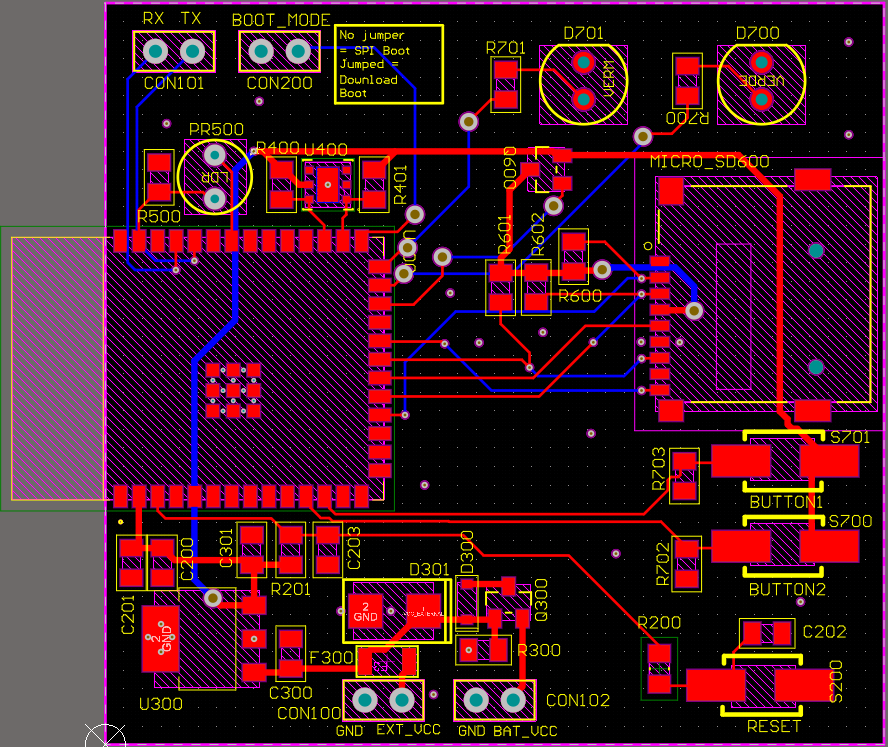
\includegraphics[width=\linewidth]{figuras/cap3/pcb/pcb_with_power.png}
            \source{Elaborado pelo autor}
        \end{figure}


    \end{columns}

    }


    \only<7>{

        \begin{block}{Plano de Terra}
            Propicia o menor caminho de retorno possível
        \end{block}

        % \vspace{10pt}

        \begin{columns}
        % \begin{figure}
            
    
            % \begin{subfigure}{0.5\linewidth}
                \column{0.45\linewidth}
                \centering
                % \vspace{3pt}
                \captionof{figure}{Top Plane}
                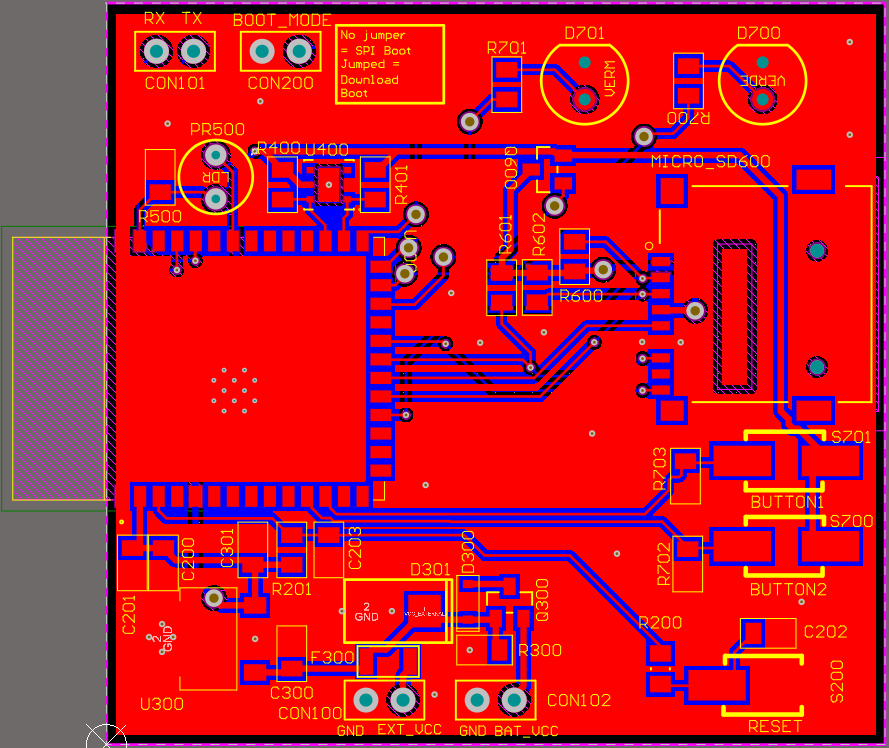
\includegraphics[width=\linewidth]{figuras/cap3/pcb/pcb_top_plane.png}
                % \source{Elaborado pelo autor}
            % \end{subfigure}   
            
            % \begin{subfigure}{0.5\linewidth}
                \column{0.45\linewidth}
                \centering
                % \vspace{3pt}
                \captionof{figure}{Bottom Plane}
                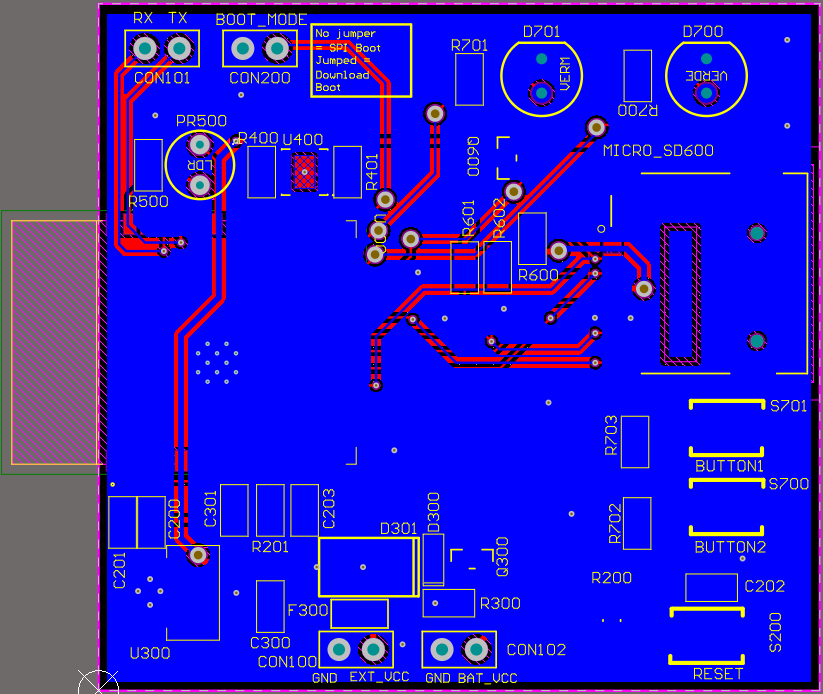
\includegraphics[width=\linewidth]{figuras/cap3/pcb/pcb_bottom_plane.png}
                % \source{Elaborado pelo autor}
                
            % \end{subfigure}

            % \source{Elaborado pelo autor}
        % \end{figure}
        \end{columns}

        \begin{figure}
            \centering
            \source{Elaborado pelo autor}
        \end{figure}

    }
    
    
    
    
    
\end{frame}

\section{Resultados}






\begin{frame}{Produção - Lista de materiais}


	\begin{table}[!h]
	\captionsetup{width=9cm}%Deixe da mesma largura que a tabela
	\caption{\label{tab:custos_fabricacao} Custo de materiais por unidades}%
% 	
		\begin{tabular}{cccc}
			\toprule
			Quantidade & Custo de Materiais  \\
			\midrule \midrule
			50 &  US\$ 502,60  \\
			100 &  US\$ 938,41 \\
			1000 & US\$ 8.736,80  \\
			\bottomrule
		\end{tabular}%
% 	}
	{%
	
% 	\Nota{esta é uma nota, que diz que os dados são baseados na
% 		regressão linear.}%
% 	\Nota[Anotações]{uma anotação adicional, seguida de várias outras.}%
    }
    
    \tiny{o autor.}%
    \end{table}    

\end{frame}


\begin{frame}{Produção - Fabricação - Custo unitário}


	\begin{table}[!h]
	\captionsetup{width=9cm}%Deixe da mesma largura que a tabela
	\caption{\label{tab:custos_montagem} Custos de fabricação e montagem JLCPCB}%
% 	
		\begin{tabular}{cccc}
			\toprule
			Quantidade & Fabricação & Montagem & Total \\
			\midrule \midrule
			50 &  US\$ 22,4 & US\$ 64,47 & US\$ 86,87 \\
			100 &  US\$ 34,4 & US\$ 96,97 & US\$ 131,37 \\
			1000 & US\$ 249,70 & US\$ 447,92 & US\$ 667,62 \\
			\bottomrule
		\end{tabular}%
% 	}
	{%
	
% 	\Nota{esta é uma nota, que diz que os dados são baseados na
% 		regressão linear.}%
% 	\Nota[Anotações]{uma anotação adicional, seguida de várias outras.}%
    }
    
    \tiny{o autor.}%
    \end{table}



    \begin{table}[!h]
	\captionsetup{width=7cm}%Deixe da mesma largura que a tabela
	\caption{\label{tab:custos_fabricacao_unitário} Custos de total unitário}%
% 	
		\begin{tabular}{cccc}
			\toprule
			Quantidade & Custo Total & Custo Unitário  \\
			\midrule \midrule
			50 &  US\$ 582,42 & US\$ 11,65 \\
			100 &  US\$ 1048,93 & US\$ 10,49  \\
			1000 & US\$ 9261,29 & US\$ 9,26  \\
			\bottomrule
		\end{tabular}%
% 	}
	{%
	
% 	\Nota{esta é uma nota, que diz que os dados são baseados na
% 		regressão linear.}%
% 	\Nota[Anotações]{uma anotação adicional, seguida de várias outras.}%
    }
    
    \tiny{o autor.}%
    
    \end{table}




\end{frame}




\begin{frame}{Produção - custo frete}

	\begin{table}[!h]
	\captionsetup{width=9cm}%Deixe da mesma largura que a tabela
	\caption{\label{tab:custos_transporte} Custos de transporte para o Brasil}%
% 	
		\begin{tabular}{cc}
			\toprule
			Quantidade & Valor  \\
			\midrule \midrule
			50 &  US\$ 80,36   \\
			100 &  US\$ 110,52 \\
			1000 & US\$ 524,49 \\
			\bottomrule
		\end{tabular}%
% 	}
	{%
	\tiny{o autor.}%
	}
	\end{table}



\end{frame}

\begin{frame}{Produção - Custos de Importação}

	\begin{table}[!h]
	\captionsetup{width=10cm}%Deixe da mesma largura que a tabela
	\caption{\label{tab:custos_importacao} Custos de importação para o Brasil}
% 	
		\begin{tabular}{ccccccccc}
			\toprule
			Quantidade & Valor & Frete & IPI & PIS & COFINS & ICMS & Total & Valor Unitário  \\
			\midrule \midrule
            50   & 2.576,22  & 412,35   & 38,85  & 62,76  & 288,40   & 741,64    & 4.120,22  & 82,40 \\
            100  & 4.815,26  & 567,11   & 69,97  & 113,03 & 519,40   & 1.335,68  & 7.420,46  & 74,20 \\
            1000 & 44.831,14 & 2.691,32 & 617,79 & 997,97 & 4.585,92 & 11.793,10 & 65.517,24 & 65,52\\
			\bottomrule
		\end{tabular}%
% 	}
	{%
	\tiny{o autor.}%
	}
	\end{table}



    
\end{frame}

\subsection{Energia}
\begin{frame}{Energia}

	\begin{table}[!h]
	\captionsetup{width=9cm}%Deixe da mesma largura que a tabela
	\caption{\label{tab:consumos_circuitos} Consumo por circuito em uso ativo}%
% 	
		\begin{tabular}{cc}
			\toprule
			Circuito & Consumo \\
			\midrule \midrule
			Controle  &  30  mA \\
			Sensores  &  27 mA  \\
			Circuito microSD   &   100 mA\\
			Interface de Usuário & 60 mA\\
		    \bottomrule
		\end{tabular}%
% 	}
	{%
	\tiny{o autor.}%
% 	\Nota{esta é uma nota, que diz que os dados são baseados na
% 		regressão linear.}%
% 	\Nota[Anotações]{uma anotação adicional, seguida de várias outras.}%
    }
    \end{table}

	\begin{table}[!h]
	\captionsetup{width=9cm}%Deixe da mesma largura que a tabela
	\caption{\label{tab:consumos_sono_profundo} Consumo por circuito em sono profundo}%
% 	
		\begin{tabular}{cc}
			\toprule
			Circuito & Consumo \\
			\midrule \midrule
			Controle  &  8 $\mu$A \\
			Sensores  &  0,2 $\mu$A  \\
			Regulador de tensão  & 65 $\mu$A\\
			Circuito microSD & 450$\mu$A \\
			Interface de Usuário & 0 $\mu$A \\
		    \bottomrule
		\end{tabular}%
% 	}
	{%
	\tiny{o autor.}%
% 	\Nota{esta é uma nota, que diz que os dados são baseados na
% 		regressão linear.}%
% 	\Nota[Anotações]{uma anotação adicional, seguida de várias outras.}%
    }
    \end{table}


    
\end{frame}


\begin{frame}{Comparativo de mercado}
    
    \begin{table}[!h]
    	
    	\captionsetup{width=9cm}%Deixe da mesma largura que a tabela
    	\caption{\label{tab:compara_dimensoes} \textit{Comparativo: Dimensões e Autonomia}}%
    % 	\resizebox{\textwidth}{!}{
    	
    		\begin{tabular}{cccc}
    			\toprule
    			Modelo & Dimensões & Nível de Proteção  & Autonomia \\
    			\midrule \midrule
               RCW-360           & Não informado   & IP64/IP65 & 3 meses       \\
               EL-WiFi-TH        & 82 x 70 x 23 mm & IP55  &6 meses       \\
               TandD RTR-507B    & 62 x 47 x 19 mm & IP64  &10 meses      \\
               160 TH            & 76 x 64 x 22 mm & IP20  & Não informado \\
               Hardware Proposto & 51 x 53 x 25 mm & Não possui & 2 meses  \\
    	    \bottomrule
    		\end{tabular}%
    % 	}{%
    	\tiny{o autor.}%

    \end{table}

    



    
\end{frame}





\begin{frame}{Comparativo - Precisão}


\begin{table}[!h]
	
	\captionsetup{width=9cm}%Deixe da mesma largura que a tabela
	\caption{\label{tab:compara_precisao} \textit{Comparativo: Faixa de leitura e Precisão}}%
% 	\resizebox{\textwidth}{!}{
	
		\begin{tabular}{ccccccc}
			\toprule
			Modelo & Faixa de Leitura (ºC) & Precisão (ºC) & Umidade Relativa (\%) & Precisão(\%)\\
			\midrule \midrule
           RCW-360           & -35 a 80      & 0,5 & 0 a 99 & 5    \\
           EL-WiFi-TH        & -20 a 60      & 0,3 & 0 a 100 & 2    \\
           TandD RTR-507B    & -25 a 70      & 0,3 & 0 a 99  & 2,50 \\
           160 TH            & -30 a 50      & 0,1 & 0 a 100 & 2 \\
           Hardware Proposto & -20 a 85      & 0,4 & 0 a 100 & 2\\
	    \bottomrule
		\end{tabular}%

	\tiny{o autor.}%

    \end{table}

    
\end{frame}





\begin{frame}{Comparativo - Preço Unitário}

    \begin{table}[!h]
	
	\captionsetup{width=7cm}%Deixe da mesma largura que a tabela
	\caption{\label{tab:compara_custo} \textit{Comparativo: Custo unitário}}%
% 	\resizebox{\textwidth}{!}{
	
		\begin{tabular}{cc}
			\toprule
			Modelo & Valor (R\$)\\
			\midrule \midrule
           RCW-360           & 1.499,00  \\
           EL-WiFi-TH        & 1.305,14  \\
           TandD RTR-507B    & 2.242,57 \\
           160 TH            & 2.842,00  \\
           Hardware Proposto & 65,52  \\
	    \bottomrule
		\end{tabular}%

	\tiny{o autor.}%

    % }
    \end{table}    
    
    
    \begin{table}[!h]
	
	\captionsetup{width=7cm}%Deixe da mesma largura que a tabela
	\caption{\label{tab:custos_extras} \textit{Comparativo: Custo unitário revisado}}%
% 	\resizebox{\textwidth}{!}{
	
		\begin{tabular}{cc}
			\toprule
			Modelo & Valor (R\$)\\
			\midrule \midrule
           RCW-360           & 1.499,00  \\
           EL-WiFi-TH        & 1.305,14  \\
           TandD RTR-507B    & 2.242,57 \\
           160 TH            & 2.842,00  \\
           Hardware Proposto & 142,35  \\
	    \bottomrule
		\end{tabular}%
	
	\tiny{o autor.}%

    \end{table}
    
\end{frame}

%% ---------------------------------------------------------------------------

% \begin{frame}{Criando Blocos}

% \end{frame}

\section{Conclusão}


\begin{frame}
    
    \centering
    \color{blue_theme}\huge{{Conclusão}}

\end{frame}


\begin{frame}{Conclusão}
    
    \begin{block}{Objetivos}
        Objetivos atingidos
    \end{block}

    \begin{block}{Trabalhos Futuros}

        \begin{itemize}
            \item Desenvolvimento de \textit{firmware} que
            faça uso dos recursos de hardware do dispositivo
            e do módulo microcontrolador;

            \item Testes com protótipos para verificar o 
            consumo energético real do dispositivo.


        \end{itemize}

        
    \end{block}




\end{frame}




\begin{frame}{}
    \centering
    \huge{\example{Obrigado.}}
    
    \vspace{1cm}
    
    % \Large{\textbf{Contato:}}
    % \newline
    % \vspace*{0.5cm}
    % \large{\email{usuario@dominio}}
\end{frame}


\section{Imagens}
\begin{frame}{Seção III - Figures}
    \begin{figure}
        \centering
        \caption{Emblema da UFC.}
        
\includegraphics[scale=0.3]{libs/emblemufc.pdf}
        \source{Obtido pelo site oficial da UFC \cite{siteufc} \cite{einstein}}
        \label{fig:ufc_emblem}
    \end{figure}
\end{frame}

%% ---------------------------------------------------------------------------
% Reference frames
\begin{frame}[allowframebreaks]
    \frametitle{Referências}
    \printbibliography
\end{frame}

%% ---------------------------------------------------------------------------
% Final frame
\begin{frame}{}
    \centering
    \huge{\textbf{\example{Obrigado(a) pela Atenção!}}}
    
    \vspace{1cm}
    
    \Large{\textbf{Contato:}}
    \newline
    \vspace*{0.5cm}
    \large{\email{usuario@dominio}}
\end{frame}


\end{document}